\documentclass{article}

% Language setting
\usepackage[english]{babel}

% Set page size and margins
\usepackage[letterpaper,top=2cm,bottom=2cm,left=3cm,right=3cm,marginparwidth=1.75cm]{geometry}

% Useful packages
\usepackage{amsmath}
\usepackage{amssymb}
\usepackage{graphicx}
\usepackage{float}
\usepackage[most]{tcolorbox}

% Bibliography
\usepackage[backend=biber, style=authoryear, sorting=ydnt]{biblatex}
\addbibresource{bibliography.bib}

% Hyperlinks (load last)
\usepackage[colorlinks=true, allcolors=blue]{hyperref}
\usepackage[capitalize]{cleveref}  % <-- subito dopo hyperref

% Code highlighting
\usepackage{minted}

% Custom command
\newcommand{\authornote}{
Mathematical principles behind it date back to \textcite{kelley1960} and one of the earliest known implementations of backpropagation can be traced back to \textcite{werbos1974}, an aerospace engineer who introduced the concept in his 1974 Ph.D. thesis at Harvard University titled "Beyond Regression: New Tools for Prediction and Analysis in the Behavioral Sciences." Werbos recognized that this algorithm could be applied not only to neural networks but to a broader range of predictive models. Despite this early insight, his work remained largely unnoticed by the mainstream AI community for nearly a decade.}

% Title and author
\title{A Primer on Backpropagation with a Numerical Example, Diagrams and Python Code }
\author{Nicola Santi}


\begin{document}
\maketitle

\begin{abstract}
A self-contained introduction to the well-known backpropagation algorithm illustrated step by step, providing the mathematical elements necessary for understanding and a numerical example with which to verify what has been learned. A Python script with Keras and TensorFlow to verify the calculations performed completes the exposition (available on \href{https://github.com/nicolinux72/backpropagation.git}{GitHub}).

\end{abstract}

\section{Introduction}
Backpropagation, short for \textit{backward propagation of errors}, is perhaps the most iconic algorithm of modern machine learning. Suffice it to say that, until the mid-1980s, no one believed in the possibility of training a multilayer network anymore! The story is very interesting and reveals how a mistaken belief can delay scientific development even by decades. \\

Although the first simple artificial neural network dates back to \textcite{mcculloch43a}, it was with \textcite{rosenblatt1962principles} that the theory and hardware needed to implement the first neural network called \textit{perceptron} were developed. The hardware needed to implement it is depicted in the photos below where we can also see Charles Wightman (project engineer) adjusting Mark I Perceptron:

\begin{figure}[H]
    \centering
    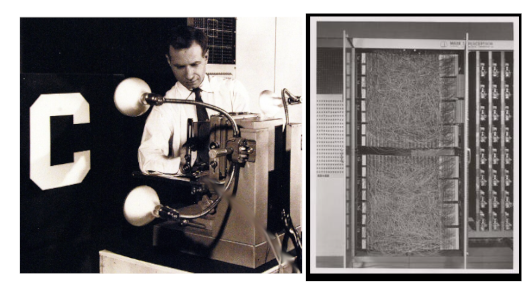
\includegraphics[width=0.8\linewidth]{images/perceptron.png}
\end{figure}


 \textit{Perceptron} has several layers but only one trainable so, in modern terms, it is a one-layer neural network, obviously subject to major limitations formally demonstrated by \textcite{minsky69perceptrons}. And here we come to the exact moment when machine learning based on neural networks was in danger of being completely abandoned because the two authors firmly believed, although without providing proof, that the same limitations of \textit{perceptron} would also apply to neural networks with more than one layer (deep learning).

 This widespread belief led to a suspension of interest, funding and research in the period from 1970 to the first half of the 1980s. Among other things, researchers could not pursue the study of multilayer models because there was no way to train them: the techniques used by \textit{perceptron} were not applicable except for networks with only one layer.

 Then, as sometimes happens, a series of innovations contributed to the revival of neural networks and, among these, the most relevant was the invention\footnote{\authornote} of the backpropagation algorithm by \textcite{rumelhart1986}. The activation and loss functions had already been made differentiable, and backpropagation allows the derivative (more precisely the gradient) of the loss function to be calculated by moving backwards from the errors (difference between the value predicted by the model and the actual value), going up from the last layer to the first. The most relevant aspect, as we shall see in this article, is the possibility of reusing the calculations already made by the neural network in its forward pass (from the first layer to the last) to calculate the gradient, which saves resources and makes it possible to handle even very deep neural networks.\\

 We will begin our exposition by recalling the few elements of mathematics necessary for understanding, which are limited to the multiplication of matrices and vectors and the calculation of derivatives of linear functions. We will then formally define a multilayer neural network and focus on a numerical example with two layers. We will use what we have learned to obtain two simple and important derivatives to be used in the last paragraph to obtain the complete backpropagation algorithm. We will test our understanding through some elementary calculations on the example model, followed by a short Python script to verify their correctness.

Let us proceed, then \verb|:-)|


\section{Matrix multiplication (and little else)}\label{sec:matrix}
In this article, we will use the original representation of matrix multiplication $WZ=A$ you can see below:

\begin{figure}[H]
    \centering
    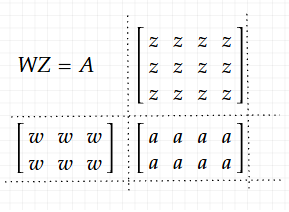
\includegraphics[width=0.3\linewidth]{images/matrix.png}
    \caption{Matrix multiplication}
\end{figure}

The advantage is the immediate visualization of the dimensions of the resulting matrix, which will have as many rows as $W$ and as many columns as $Z$. Recall also that the number of columns of $W$ must coincide with the number of rows of $Z$ for multiplication to occur.

Let us now look at the special case of multiplication between matrix and vector $W\boldsymbol{z}=\boldsymbol{a}$:

\begin{figure}[H]
    \centering
    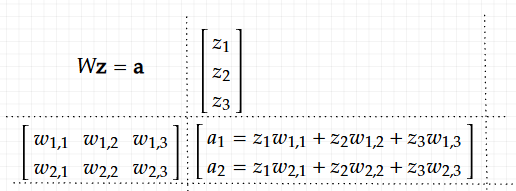
\includegraphics[width=0.5\linewidth]{images/matrix-vector.png}
    \caption{Matrix and vector multiplication}
    \label{fig:enter-label}
\end{figure}

It is important to note how each element of $\boldsymbol{z}$ contributes to determining each element of $\boldsymbol{a}$. This awareness will be useful in one of the final sections of this paper (\ref{sec:meet-delta}). Moreover, this is precisely why layers involving matrix multiplication are called dense: each input element influences every output element.

Finally, each $a_k$ being the sum of products between elements of $\boldsymbol{z}$ and $W$, the derivative of $a_k$ with respect to $z_m$ is simply $w_{k,m}$ while, symmetrically, the derivative with respect to $w_{k,m}$ is $z_m$ (see \ref{sec:same-layer}).

\section{Multilayer dense network: formalization}
A dense feedforward neural network can be formalized as a sequence of $\displaystyle L$ layers, each of which receives an input vector $\displaystyle \mathbf{z} \in \mathbb{R}^{M}$ to which it first applies a linear transformation $\displaystyle W$ and then a nonlinear transformation $\displaystyle h()$. The result is used by the next layer as input (hence the feedforward meaning), see Figure below.

\begin{figure}[H]
    \centering
    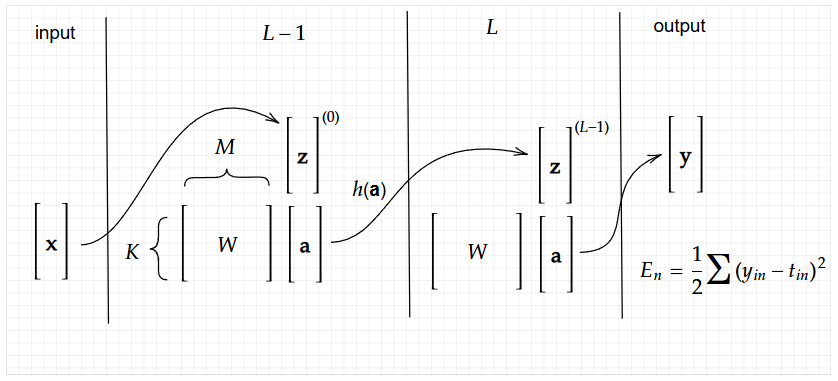
\includegraphics[width=0.8\linewidth]{images/multi layers network.png}
    \caption{Simple feedforward network}
    \label{fig:multi-layer-network}
\end{figure}

The linear transformation inside each layer multiplies the input vector $\displaystyle \mathbf{z}$ by the model parameter $\displaystyle K\times M$ matrix $\displaystyle W$ (each layer has its own matrix with different dimensions $M$ and $K$) so that each input neuron (each component of vector $\displaystyle \mathbf{z}$) is connected to each output neuron (component of vector $\displaystyle \mathbf{a}$). The result is the vector $\displaystyle \mathbf{a} \in \mathbb{R}^{K}$.

\begin{figure}[H]
    \centering
    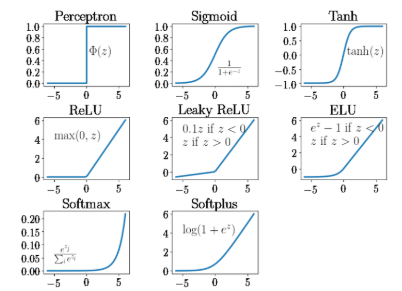
\includegraphics[width=0.6\linewidth]{images/activation functions.png}
    \caption{Some common activation functions}

\end{figure}

A potentially nonlinear transformation called activation function is then applied to vector $\displaystyle \mathbf{a}$. Common examples of this kind of function are softmax, ReLU or sigmoid (see Figure above from \url{www.researchgate.net}). In turn, the result of this activation function becomes the input of the next layer $\displaystyle \mathbf{z}^{( l)} =h(\mathbf{a}^{( l)})$. The superscripts in parentheses indicate the layer to which each variable refers.

Summarizing and formalizing, for each layer $\displaystyle l$ we have:

\begin{gather*}
\mathbf{a}^{( l)} =W^{( l)}\mathbf{z}^{( l-1)}\\
\mathbf{z}^{( l)} =h^{( l)}\left(\mathbf{a}^{( l)}\right)\\
M^{( l)}=K^{( l-1)} \
\end{gather*}

The loss function (also known as error function) is simply the mean square of the errors $E_{n}(\mathbf{y}) =\frac{1}{2}\sum ( y_{mn} -t_{mn})^{2}$, where $n$ denotes a single data point.   \\

A couple of definitions and a few remarks conclude the presentation of our network:
\begin{itemize}
    \item $\displaystyle \mathbf{x} =\mathbf{z}^{( 0)}$   is the input of the whole neural network;
    \item $\displaystyle \mathbf{y} =\mathbf{z}^{( L)}$  is the output of the whole neural network;
    \item $\displaystyle L$ is the total number of layers;
    \item $\displaystyle M^{( l)}$ is the dimension of layer $l$ input $\displaystyle \mathbf{z}^{( l-1)} \in \mathbb{R}^{M^{( l)}}$;
    \item $\displaystyle K^{( l)}$ is the dimension of the layer $l$ output $\displaystyle \mathbf{z}^{(l)} \in \mathbb{R}^{K^{( l)}}$;
    \item $ K^{( l-1)}=M^{(l)} \ $ obviously, the size of the output of each layer must match the next layer input. The last three equalities will be particularly useful in paragraph \ref{sec:from-previous};
\end{itemize}
\

\begin{tcolorbox}[colback=gray!10, colframe=gray!50, title=Note]
For didactic purposes, the last layer $L$ has no activation function or, equivalently, uses the identity function $h(\boldsymbol{a})=\boldsymbol{a}$. We will return to this point in section \ref{sec:last-layer}.
For similar reasons, each layer has no bias.
\end{tcolorbox}

The superscripts in parentheses, as mentioned, indicate the layer to which each variable refers: they are somewhat inconvenient, so, for simplicity, in case of omission it will be understood that we are referring to the current layer $\displaystyle l$. So we can simplify our equations:

\begin{gather*}
\mathbf{a} =W\mathbf{z}^{( l-1)}\\
\mathbf{z} =h(\mathbf{a})\\
M=K^{( l-1)} \
\end{gather*}

\textbf{Python code:} we can declare the model just described with a few lines of Python using the well-known Keras library.

\begin{tcolorbox}[colback=gray!10, colframe=gray!50, title=Model definition]
\begin{minted}{python}
model = keras.Sequential([
    layers.Input(shape=(2,)),
    layers.Dense(3, activation='tanh',   use_bias=False),
    layers.Dense(2, activation='linear', use_bias=False)
])
\end{minted}
    \end{tcolorbox}


The code is very simple: the exclusion of the bias and the activation function of the last layer, which coincides with the identity function (as if it were not there), are worth noting.

Please remember that the source code is available on \href{https://github.com/nicolinux72/backpropagation.git}{GitHub}.

\section{Four simple derivatives (in fact, only two)}

In this section, we will try to understand how $\boldsymbol{a}$ varies with respect to the variables of the same layer ($W$ and $\boldsymbol{z}$) and, subsequently, with respect to the tensor $\boldsymbol{a}^{l-1}$ of the previous layer.

We will discover that we are dealing with very simple derivatives, given the extreme linearity of the model. I recommend following the calculations in the figure below.

\begin{figure}[H]
    \centering
    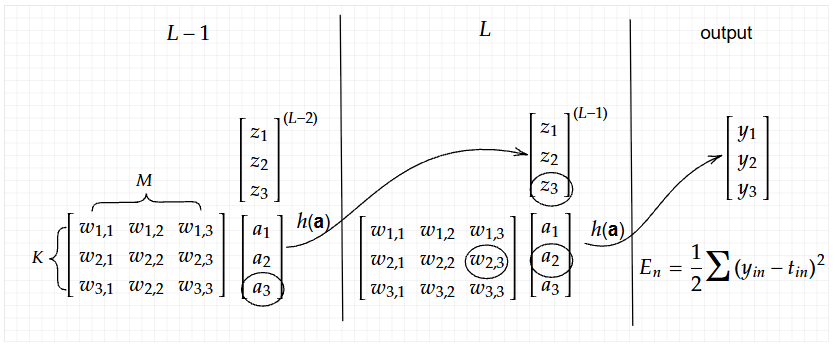
\includegraphics[width=0.8\linewidth]{images/last-layers details.png}
    \caption{Derivatives of $\boldsymbol{a}$ with respect to the current layer $L$ and the previous one}
    \label{fig:last-details}
\end{figure}


\subsection{Inside same layer}\label{sec:same-layer}

In each layer $\displaystyle l$ we have two simple derivatives to deal with:

\begin{gather}
\frac{\partial a_{k}}{\partial w_{k,m}} \ =\ z_{m}^{( l-1)} \label{eq:from-w}\ \ \\
\notag\\
\frac{\partial a_{k}}{\partial z_{m}^{( l-1)}} \ =\ w_{k,m} \label{eq:from-z} \ \
\end{gather}

Taking as a reference the circled elements in Figure \ref{fig:last-details}: we know from paragraph \ref{sec:matrix} that $\displaystyle a_{2} =w_{2,1} z_{1} +\ w_{2,2} z_{2} +\ w_{2,3} z_{3}$ so the derivative of $ a_2$ with respect to $\displaystyle w_{2,3}$ is simply $\displaystyle z_{3}$. Or, conversely, the derivative of $\displaystyle a_{2}$ with respect to $\displaystyle z_{3}$ is  $\displaystyle w_{2,3}$.\\

\textbf{Note}: equation \eqref{eq:from-z}, upon closer inspection, already connects to the previous layer being the input of layer $\displaystyle l$ the output of the previous one, but it is not yet the derivative with respect to $\boldsymbol{a}^{l-1}$ that we will calculate in the next paragraph.\\

\begin{figure}[H]
    \centering
    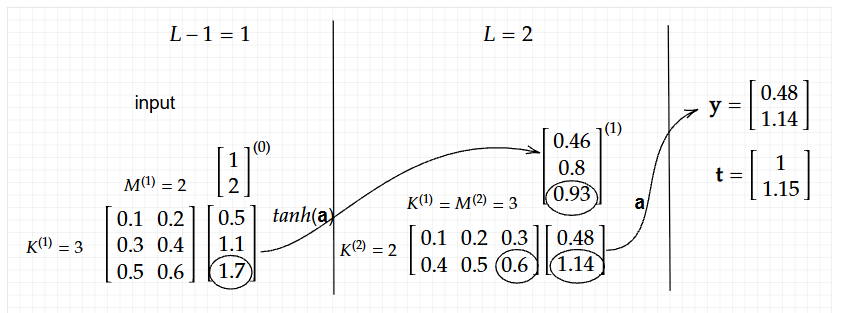
\includegraphics[width=0.8\linewidth]{images/example.png}
    \caption{A numerical example}
    \label{fig:example}
\end{figure}

\textbf{Our example:} to refine our understanding, let us use the small two-layer neural network drawn above. The weights displayed are those at a certain epoch in training, the label $\boldsymbol{t}$ is the truth value for a certain data point. All values are approximated to two decimal places. Now, referring to layer 2, we calculate the partial derivatives of $a_2$.


\begin{gather}
\frac{\partial a_{2}}{\partial w_{2,3}} \ =\ z_{3}^{( 1)} =0.93 \notag  \\
\notag\\
\frac{\partial a_{2}}{\partial z_{3}^{( 1)}} \ =\ w_{2,3} \ =\ 0.6 \notag
\end{gather}

\begin{center}\textleaf\end{center}

\textbf{Python code:} we can recreate our example by initializing the weights of each layer, instantiating the $x$ input tensor and the $t$ label.

\begin{tcolorbox}[colback=gray!10, colframe=gray!50, title=Parameters initialization]
\begin{minted}{python}
# set weights as in the article
w1 = np.array([[0.1, 0.2],
               [0.3, 0.4],
               [0.5, 0.6]])

w2 = np.array([[0.1, 0.2, 0.3],
               [0.4, 0.5, 0.6]])

model.layers[0].set_weights([w1.T])
model.layers[1].set_weights([w2.T])

# set also a fake data point and label
x = tf.constant([[1.0, 2.0]])
y_true = tf.constant([[1.0, 1.15]])
\end{minted}
\end{tcolorbox}


\subsection{From previous layer}\label{sec:from-previous}
As noticed, derivative \eqref{eq:from-z} already links the current layer to the previous one, because $\displaystyle \mathbf{z}^{( l-1)}$ is both the previous layer output and the current layer input. But we need to be linked to previous $\boldsymbol{a}^{l-1}$. It's an easy task remembering that $\displaystyle \ z_{m}^{( l-1)} =h^{( l-1)}( a_{m}^{( l-1)})$, so:


\begin{gather}
\frac{\partial z_{m}^{( l-1)}}{\partial a_{m}^{( l-1)}} \ =\dot{h}^{( l-1)} (a_{m}^{(l-1)})\label{eq:prev}
\end{gather}

This, obviously, involves $\dot{h}^{l-1}()$, the derivative of activation function $h^{l-1}()$. If you are surprised by the use of the same index $m$ to refer to vectors of different layers, $z^{(l-1)}$ after all lies in layer $l$ while $a^{(l-1)}$ lies in $l-1$, just take a look at Figure \ref{fig:multi-layer-network} and remember that $M^{(l)}=K^{(l-1)}$.   \\

\textbf{Our example:} Again, using Figure \ref{fig:example}, we calculate the derivative of the third component of the first-layer output $z_{3}^{( 1)}$ (which is also the third component of the second-layer input) with respect to $a_{3}^{( 1)}$. Remember that, in our example, the activation of layer $L-1$ is $\tanh()$ and that the derivative of $\tanh()$ is precisely $1-\tanh^2()$:

\begin{equation*}
\frac{\partial z_{3}^{( 1)}}{\partial a_{3}^{( 1)}} \ =\dot{\tanh}( 1.7) =1-\tanh^{2}( 1.7) =1-( 0.93)^{2}=0.14
\end{equation*}

\begin{center}\textleaf\end{center}


We have developed the necessary formulas to finally calculate the derivative of \textbf{each single component} of $\boldsymbol{a}$ with respect to each $a_m^{(l-1)}$ of the previous layer using equations \eqref{eq:from-z} and \eqref{eq:prev}:

\begin{gather}
\frac{\partial a_{k}^{(l)} }{ \partial a_{m}^{( l-1)}}
= \underbrace{\frac{\partial z_{m}^{( l-1)}}{\partial a_{m}^{( l-1)}}}_{\eqref{eq:prev}} \
\underbrace{\frac{\partial a_{k}^{( l)}}{\partial z_{m}^{( l-1)}}}_{\eqref{eq:from-z}} \
=\dot{h}^{( l-1)}( a_{m}^{( l-1)}) \ w_{k,m}^{( l)} \label{eq:a-prev}
\end{gather}\\

As in \eqref{eq:prev}, $m$ and $k$ refer both to layer $l$.\\

\textbf{Our example:} we simply apply equation \eqref{eq:a-prev}


\begin{equation*}
\frac{\partial a_{2}^{( 2)}}{\partial a_{3}^{( 1)}} \  = (0.14)\ 0.6 = 0.084
\end{equation*}

In conclusion, we will only need a couple of derivatives from this paragraph, namely equations \eqref{eq:from-w} and \eqref{eq:a-prev}.

\section{Backpropagation algorithm}
To train our model we need to compute the derivative (more precisely the gradient) of each loss function $\displaystyle E_{n}(\mathbf{y}) =\frac{1}{2}\sum ( y_{in} -t_{in})^{2}$ with respect to all model parameters $w_{k,m}$.

\begin{figure}[H]
    \centering
    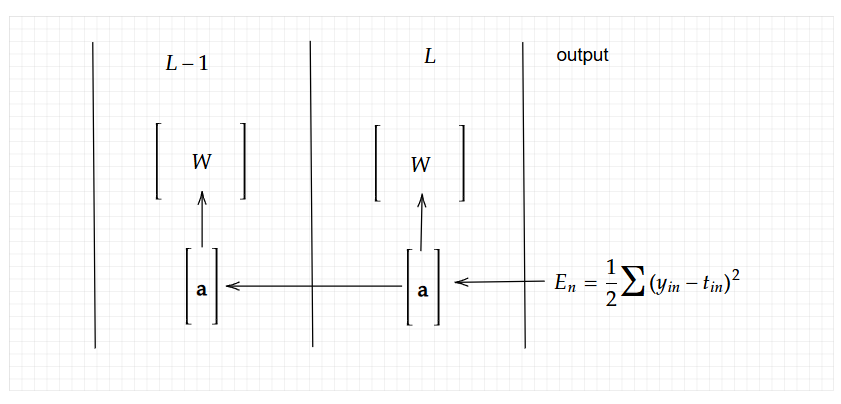
\includegraphics[width=0.6\linewidth]{images/backprop.png}
    \caption{Backpropagation moves from layer to previous one using $\boldsymbol{a}$ derivatives and then computes gradient with respect to $W$.}
    \label{fig:a-to-a}
\end{figure}


The basic idea of backpropagation is to calculate the derivative of $E$ with respect to all $\boldsymbol{a}$ starting from the last layer $L$ and proceeding backward using \eqref{eq:a-prev}. Moreover, as we will see, moving in reverse we can reuse the calculations already made during the forward pass.

\subsection{Meet $\delta$, the propagated error}\label{sec:meet-delta}

The full name of the algorithm that is the object of this article is \textit{backward propagation of errors}, referring precisely to the errors of the model output, which are also the individual components of the loss function. Let us meet $\boldsymbol{\delta}$ for the last layer:


\begin{equation}
\delta _{k}^{( L)} =y_{k} -t_{k} \label{eq:last-error}
\end{equation}

You could note that it is precisely the difference between the $k$-th component of the model output $\boldsymbol{y}$ and the correct value $\boldsymbol{t}$, so we could call $\boldsymbol{\delta}$ simply \textit{errors} and define it formally for each layer:


\begin{equation}
\delta _{k}^{( l)} \equiv \frac{\partial E}{\partial a_{k}^{( l)}} \label{eq:error}
\end{equation}

It is simply the partial derivative of the loss function with respect to a component of $\boldsymbol{a}$. Remember from Figure \ref{fig:a-to-a} that backpropagation uses these intermediate derivatives to reach its ultimate goal: the derivative of $E$ with respect to each $W$.

Finally, that equation \eqref{eq:error}, in the last layer, coincides with equation \eqref{eq:last-error} is easily demonstrated:

\begin{equation*}
\frac{\partial E}{\partial a_{k}^{( L)}}
=\frac{\partial \frac{1}{2}\sum ( a_{i} -t_{i})^{2}}{\partial a_{k}^{( L)}}
=\frac{\partial \frac{1}{2}\sum ( y_{i} -t_{i})^{2}}{\partial a_{k}^{( L)}}
=\ y_{k} -t_{k}
\end{equation*}


\begin{tcolorbox}[colback=gray!10, colframe=gray!50, title=Please note:]
As mentioned, in our simplified model the last layer has no activation function: if there were one, it would have to be taken into account in exactly the same way as equation \eqref{eq:prev}, but the interpretation of $\boldsymbol{\delta}$ as closely related to the error measure would remain valid.
\end{tcolorbox}

\textbf{Our example:} Let's calculate the error $\boldsymbol{\delta}^{L}$ of our example, please return to Figure \ref{fig:example}:


\begin{gather*}
\delta _{1}^{( 2)} =\frac{\partial E}{\partial a_{1}^{( 2)}} \ =\ ( 0.48-1) \ =-0.52\ \ \\
\\
\delta _{2}^{( 2)} =\frac{\partial E}{\partial a_{2}^{( 2)}} \ =\ ( 1.14-1.15) \ =-0.01
\end{gather*}

\begin{center}\textleaf\end{center}


Equation \eqref{eq:a-prev} connects each component of $\boldsymbol{a}^{(l)}$ with each component of $\boldsymbol{a}^{(l-1)}$, but the calculation of $\boldsymbol{\delta}^{(l)}$ for the layers preceding the last one requires us to give additional thought: $E$ depends on all the components of $\boldsymbol{a}^{(l)}$ (not just one), so we will have to take into account (by adding them up) all these variations.

Remembering paragraph \ref{sec:matrix} and with the help of Figure \ref{fig:example}, we obtain:

\begin{gather*}
\delta _{m}^{( L-1)} =\frac{\partial E}{\partial a_{m}^{( L-1)}} \ =\sum _{k}^{K^{( L)}}
\underbrace{\frac{\partial z_{m}^{( L-1)}}{\partial a_{m}^{( L-1)}}\frac{\partial a_{k}^{( L)}}{\partial z_{m}^{( L-1)}}}_{\eqref{eq:a-prev}} \
\underbrace{\frac{\partial E}{\partial a_{k}^{( L)}}}_{\eqref{eq:error}}\\
\\
=\dot{h}^{( L-1)}\left( a_{m}^{( L-1)}\right)\sum _{k}^{K^{( L)}} \ w_{k,m}^{( L)} \ \delta _{k}^{( L)} \ \ \\
\end{gather*}

We have used equations \eqref{eq:a-prev} and \eqref{eq:error} where indicated. As before, $m$ and $k$ refer to layer $L$.

\textbf{Our example:} I think it may be useful to train intuition with the simple calculations for the penultimate $L-1$ layer (which, in our example, is also the first). Starting with $\boldsymbol{\delta^{L-1}}$


\begin{gather*}
\delta _{1}^{( 1)} =\dot{\tanh}( 0.5)[ \ 0.1\ ( -0.52) +\ 0.4( -0.01)] =-0.044\\
\delta _{2}^{( 1)} =\dot{\tanh}( 1.1)[ \ 0.2\ ( -0.52) +\ 0.5( -0.01)] =-0.039\\
\delta _{3}^{( 1)} =\dot{\tanh}( 1.7)[ \ 0.3\ ( -0.52) +\ 0.6( -0.01)] =-0.020
\end{gather*}

\begin{center}\textleaf\end{center}


For the sake of completeness, we report the general formula which, after our journey, I hope will no longer be intimidating:


\begin{equation}
\delta _{m}^{( l-1)} \equiv \frac{\partial E}{\partial a_{m}^{( l-1)}} \ =\begin{cases}
( y_{m} -t_{m}) & l=L\\
\dot{h}^{( l-1)}( a_{m})\sum _{k}^{K^{( l)}} \ w_{k,m}^{( l)} \ \delta _{k}^{( l)} \ \  & l< L
\end{cases} \ \ \ \ \ \ \ \ \ \ m\in \left[ 1,M^{( l-1)}\right] \label{eq:backprop}
\end{equation}


\subsection{Conclusion of propagation}

Having the (partial) derivatives with respect to $\boldsymbol{a}^{(l)}$ for each layer, it is rather simple to find the derivatives of $E$ with respect to each parameter $w_{k,m}^{l}$ and thus ultimately achieve the goal of calculating the gradient of the loss function with respect to the parameters.

We complete the calculation for the last layer by deriving $\boldsymbol{a}$ with respect to each element $W$. We are helped by equations \eqref{eq:from-w} and \eqref{eq:error}.

\begin{gather*}
\frac{\partial E}{\partial w_{k,m}^{L}}
= \frac{\partial E}{\partial a_{k}^{L}} \frac{\partial a_{k}^{L}}{\partial w_{k,m}} \ =\ \delta_k^{L} \ z_{m}^{( l-1)} \label{eq:delta-from-w}
\end{gather*}\\

\textbf{Our example:}  compute the derivative for each  $w_{k,m}$ of the last layer $L=2$


{\small
\begin{gather*}
\frac{\partial E}{\partial w_{1,1}^{( 2)}} \ =\ -0.52\ ( 0.46 ) = -0.24 \ ;\ \ \
\frac{\partial E}{\partial w_{1,2}^{( 2)}} \ =\ -0.52\ ( 0.80 ) = -0.41 \ ;\ \ \
\frac{\partial E}{\partial w_{1,3}^{( 2)}} \ =\ -0.52\ ( 0.93 ) = -0.48 \\
\\
\frac{\partial E}{\partial w_{2,1}^{( 2)}} \ =\ -0.01\ ( 0.46 ) = -0.00 \ ;\ \ \
\frac{\partial E}{\partial w_{2,2}^{( 2)}} \ =\ -0.01\ ( 0.80 ) = -0.01 \ ;\ \ \
\frac{\partial E}{\partial w_{2,3}^{( 2)}} \ =\ -0.01\ ( 0.93 ) = -0.01
\end{gather*}
}


Now, compute the derivatives with respect to $W^{L-1}$


{\small
\begin{gather*}
\frac{\partial E}{\partial w_{1,1}^{( 1)}} \ =\ -0.044\ ( 1 ) = -0.04 \ ;\quad
\frac{\partial E}{\partial w_{1,2}^{( 1)}} \ =\ -0.044\ ( 2 ) = -0.09 \ ;\\
\\
\frac{\partial E}{\partial w_{2,1}^{( 1)}} \ =\ -0.039\ ( 1 ) = -0.04 \ ;\quad
\frac{\partial E}{\partial w_{2,2}^{( 1)}} \ =\ -0.039\ ( 2 ) = -0.08 \ ;\\
\\
\frac{\partial E}{\partial w_{3,1}^{( 1)}} \ =\ -0.020\ ( 1 ) = -0.02 \ ;\quad
\frac{\partial E}{\partial w_{3,2}^{( 1)}} \ =\ -0.020\ ( 2 ) = -0.04
\end{gather*}
}

 Please note that we have calculated the derivatives with respect to all weights using only values already computed during the forward pass of the network, from the first layer to the last.

\section{Checking the calculations}

We add code to instruct our script to perform the gradient calculation in order to check the accuracy of our results. When comparing, we take into account the rounding to two decimal digits used in our examples.


\textbf{Python code:} We calculate the gradient using the self-differentiation of TensorFlow.

\begin{tcolorbox}[colback=gray!10, colframe=gray!50, title=Gradient calculation]
\begin{minted}{python}
# setup auto-differentiation
with tf.GradientTape() as tape:
    y_pred = model(x)                                     # Forward pass
    loss = tf.reduce_mean(tf.square(y_true - y_pred))     # MSE (L2)

# Compute gradient
grads = tape.gradient(loss, model.trainable_variables)

# show gradients for our datapoint (direct)
print("--- Input:", x.numpy(), "\n")
print("--- Gradients")
print(f"Layer 1:\n{grads[0].numpy().T}")
print("Output:", model.layers[0](x).numpy(), "\n")
print(f"Layer 2:\n{grads[1].numpy().T}")
print("Output:", y_pred.numpy(), "\n")
print("--- Label:", y_true.numpy(), "\n")
\end{minted}
\end{tcolorbox}

 The output of the script, see the next figure, confirms our calculations to an accuracy level of more than two decimal places.

\begin{figure}[H]
    \centering
    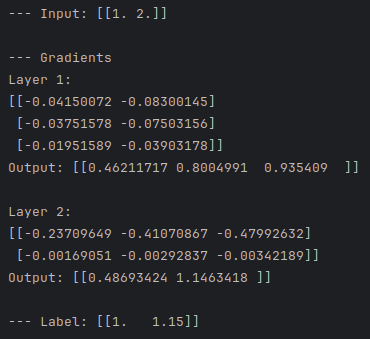
\includegraphics[width=0.5\linewidth]{images/output.png}

\end{figure}

\section{Conclusions}

In this article, we illustrated the backpropagation algorithm step by step by placing theory side by side with a small neural network used to refine intuition and carry out calculations. We did not skimp on graphs and insights, going as far as implementing a simple Python script using Keras and TensorFlow, available on \href{github.com/nicolinux72/backpropagation.git}{GitHub}.

\nocite{*}
\printbibliography


\end{document}